\section{Introduction}
\label{sec:intro}

\begin{comment}

Motivation:
- Counterfactual is important. Used in many evaluation and model improvement approaches. Like mentioned in other papers, perturbations of inputs would allow us to highlight what really matters more efficiently than getting different examples
- Existing methods have limitations:
	○ Auto-method seems to focus on word substitution, or paraphrasing. More scalable, but usually too simplistic.
	○ More diverse counterfactuals rely on human effort. More diverse and natural, but hard to scale:
		§ Cannot create this for all instances
		§ For just one instance, just getting one perturbation (good -> bad) still ignores many other decision boundary dimensions (good -> not good)
	- Goal: To create a counterfactual generator that
		○ can automatically cover more patterns
		○ But still systematic enough for scaled analysis

Contribution bullets:
	- Survey on prior work, summarize applications + desired properties
	- Perturbation as a generation model, the design of perturbation type control and the importance of [BLANK]
	- Application - counterfactual explanation
		○ Design - categorize patterns to search for, grouping/ranking/summarization, interactive mode
		○ Validly - User study
		○ Finding - case study on some model
	- Application - labeling
		○ Ranking, grouped labeling
		○ Training data: get better results compared to
			§ Adding the same amount of training data
			§ asking people to generate counterfactuals using the same budget
		○ Evaluation data: further decrease the SOTA model performance
		○ Vision - not tested, but we think presenting some existing perturbations first should help people get more creative when they come up with their owns [future work…]



The hope is that while perturbations from crowdsourced data are very task specific (e.g. trying to change the sentiment label), we can learn general templates like 'remove modifier', 'change plural to singular', etc. These perturbations can be a contribution on its own, as they can be useful for testing, data augmentation, and other tasks.

Labeling perturbed examples (2b) is much easier than labeling new examples, especially for examples in SQuAD (which requires you to parse a lot of sentences/paragraphs). That means that this makes it much easier to create contrast sets (criticism: we only get contrast examples that look like our template). 

Perturbations are more systematic, and labeling perturbed examples can potentially help create models that are more robust, generalize better, etc.

Compared to manual perturbation and labeling, the templates can potentially trigger more creative perturbations (because the naive ones are performed by the template).

\end{comment}
% 1. Define counterfactual. counterfactuals are how we understand stuff (cite psychology papers) and run decent experiments. Counterfactuals are hard in the real world (cite pearl), but easy if we're analyzing a model
% 2. Current counterfactuals in NLP: useful for training and eval (contrast sets), but done by hand. Too much work, relies on creativity, may miss stuff. For explanations: adversarial examples, or simple word substitutions.
% 3. We formalize the task of counterfactual generation: given x, produce x', and then rank according to the task. We train a model to do this (some detail).
% 4. we apply the model to training, eval, explanations. summary of results. Important: compare to counterfactuals created by hand, this is better and faster
Counterfactual reasoning (mentally simulating what \emph{would have happened} if conditions were different) is a common tool for making causality assessments \cite{kahneman}, which in turn are crucial for explanation \cite{miller}, evaluation, and learning. For example, in Figure X the sentence $x = \text{This is a good movie}$ is perturbed into various $[x'_1, x'_2, ...]$ in such a way that the link $x \rightarrow x'_i$ brings different kinds of insights by simulating what would have happened to if $x$ was different.

Applications of counterfactual reasoning to NLP generally specify what the $x \rightarrow x'$ relationship is, and then ask humans to manually create counterfactuals $x'$ or perturbation functions that generate $x'$.
For example, \citet{gardner2020contrast} and \citet{kaushik2019learning} ask humans to create counterfactuals $x'$ that are as close to $x$ as possible \emph{but have a different label}, which are in turn used to improve training and evaluation. Similarly, \citet{wu2019errudite} and \citet{checklist:acl20} ask humans to create counterfactual-generating functions such as ``remove negation'' or ``add irrelevant information'' in order to verify or test specific model behaviors (e.g. whether models handle negation appropriately).
These are costly to generate, and may miss important patterns due to their reliance on human creativity.
Another application is adversarial example generation, where the relationship between $x$ and $x'$ is semantic equivalence \emph{and} difference in model prediction\cite{iyyer2018adversarial, ribeiro2018semantically}. In this rare case where counterfactuals can reliably be produced automatically, humans are not able to produce counterfactuals with the desired property as well as automatic methods  \cite{ribeiro2018semantically}, even though they excel at evaluating such counterfactuals.
%TODO: NEed to say something about Li et al 2020 Linguistically-Informed Transformations (LIT): A Method for Automatically Generating Contrast Sets, maybe something about word substitution

In this work, we formalize the task of \emph{automatic counterfactual generation} (AGS), where given an input $x$, the goal is to produce a set of counterfactuals $[x_1, x_2, ...]$ with reasonable relationships $x \rightarrow x_i$. We frame AGS as text generation, and finetune GPT-2 \cite{radford2019language} on a dataset of $x \rightarrow x'$ pairs, such that it can generate general purpose counterfactuals. We also allow for targeted counterfactuals, by specifying where the perturbation occurs in the sentence \cite{donahue2020enabling} and using control codes such as [deletion], [lexical], or [negation] (Figure X). The produced set of counterfactuals is then ranked or filtered, depending on the task of interest.
%TODO: need a name here

We demonstrate the usefulness of NAME in three different tasks that require counterfactual reasoning: training, evaluation, and explanation. For training and evaluation, we observe that asking humans to evaluate counterfactuals (rather than the more difficult task of creating them \cite{gardner2020contrast, kaushik2019learning}) is enough to produce high-quality contrast sets \cite{gardner2020contrast} and training data that results in higher generalization accuracy (measured by out-of-domain datasets, challenge sets, contrast sets, and CheckLists \cite{checklist:acl20}).
Finally, we use NAME to produce \emph{black-box counterfactual explanations}. Research from the social sciences indicates that counterfactual contrast cases are more intuitive as explanations \cite{miller}. We run a user study that indicates that these explanations indeed are useful on their own, or as a complement to popular feature attribution methods such as SHAP \cite{NIPS2017_7062}.
% TODO: say something about gardner / kaushik in terms of efficiency or something else, improve this explanation stuff.

\section{Old Intro}

% In the context of NLP, if we have a piece of text $x$, we say that $x'$ is a counterfactual if there is a relationship $x \rightarrow x'$ such that $x'$ brings insight into $x$.


\wts{\emph{counterfactual analysis}, where one slightly modifies the input data to eliminate potential spurious feature-label correlations~\cite{jia2017adversarial, ribeiro2018semantically}.
%The intuition is, language is high dimensional, and in comparison datasets provide sparse signal.
We expect counterfactual perturbations to fulfill the gap between limited linguistic variations in
the training data and the diversity in real-world languages~\cite{tu2020empirical, kaushik2019learning}.
}
\wts{
Similarly, counterfactual attacks to models either rely on manual rewrites~\cite{kaushik2019learning, gardner2020evaluating} --- and therefore are diverse yet unscalable --- or take limited, mostly rule-based forms of word substitutions, keyword deletions, or paraphrasing~\cite{agrawal2016analyzing, mudrakarta2018did, feng2018pathologies}.
Moreover, they are mainly for the purpose of detecting over-stability or over-sensitivity.
In contrast, I am interested in generating counterfactual examples that are diverse yet systematic, for the purpose of understanding \emph{why} models behave in certain ways.
}

Researchers and practitioners expect NLP models to learn linguistic patterns, yet language is too high dimensional for any datasets to exhaust.
Due to annotation artifacts~\cite{gururangan2018annotation}, models usually learn spurious correlations that are hard to detect with test datasets, who have similar biases as the training set~\cite{rajpurkar-etal-2018-know}.
%Compared to random data, various work has found that 
To inspect and improve models' decision boundaries, various work has explored perturbing existing datasets, rather than adding new random data.
The intuition is, paired data points can more effectively reveal unlearned phenomena. 


However, these approaches have their limitations. 
Automated methods that frequently use templates~\cite{li2020linguistically}, word substitution~\cite{li-etal-2020-bert-attack} or paraphrasing~\cite{iyyer2018adversarial} are scalable, but usually cover simplistic, limited number of perturbations or do not cross models' decision boundaries.
More diverse perturbations rely on human effort~\cite{gardner2020contrast, kaushik2019learning}, but becomes hard to scale to more instances.
In fact, with prior work mostly inspecting one or two perturbations per instance, it even has limited coverage a single instance.
For example, a single perturbation changing from \remove{great} to \add{not great} still omits other decision boundary dimensions, \eg \swap{great}{could have been great},  \swap{great}{disastrous}.

In this work, we explore the automated perturbation generation.
We survey existing papers on applications of perturbations, and summarize that a perturbation generator should automatically cover various patterns, but are still controlled enough to allow targeted changes (for pattern-specific data augmentation or model analysis.)
We formalize the perturbation as a generative task, and instantiate the generator by finetuning language models.
While language models like GPT-2 are typically for fulfilling remaining sentences and paragraphs~\cite{radford2019language}, we design the training prompts such that the model learns to generate the perturbation after seeing the original sentence.

Specifically, for each pair, we generate the training prompt such that:
(1) The prompt concatenates the original sentence and the new one;  
(2) The prompt uses a fill-in-the-blank structure~\cite{donahue2020enabling}, that determines \emph{where} to change (based on linguistic features like part-of-speech tagging or dependency trees);
(3) The prompt contains \tagstrs that directs \emph{how} to change a sentence, which we summarize based on existing papers on perturbations.
To help the model learn different \tagstrs, we combine six existing datasets for the finetuning.
All datasets contain paired sentences that can be viewed as minimal perturbations of each other, but cover different \tagstrs.
As a result, in Figure~\ref{fig:teaser} to test the impact of negation, one can say \emph{``add negation modifiers to aux.''}\wts{Add figure.}
%, instead of enumerating rules like \swap{did}{didn't}, \swap{\texttt{VERB}}{would never \texttt{VERB}}

\begin{figure}[t]
\centering
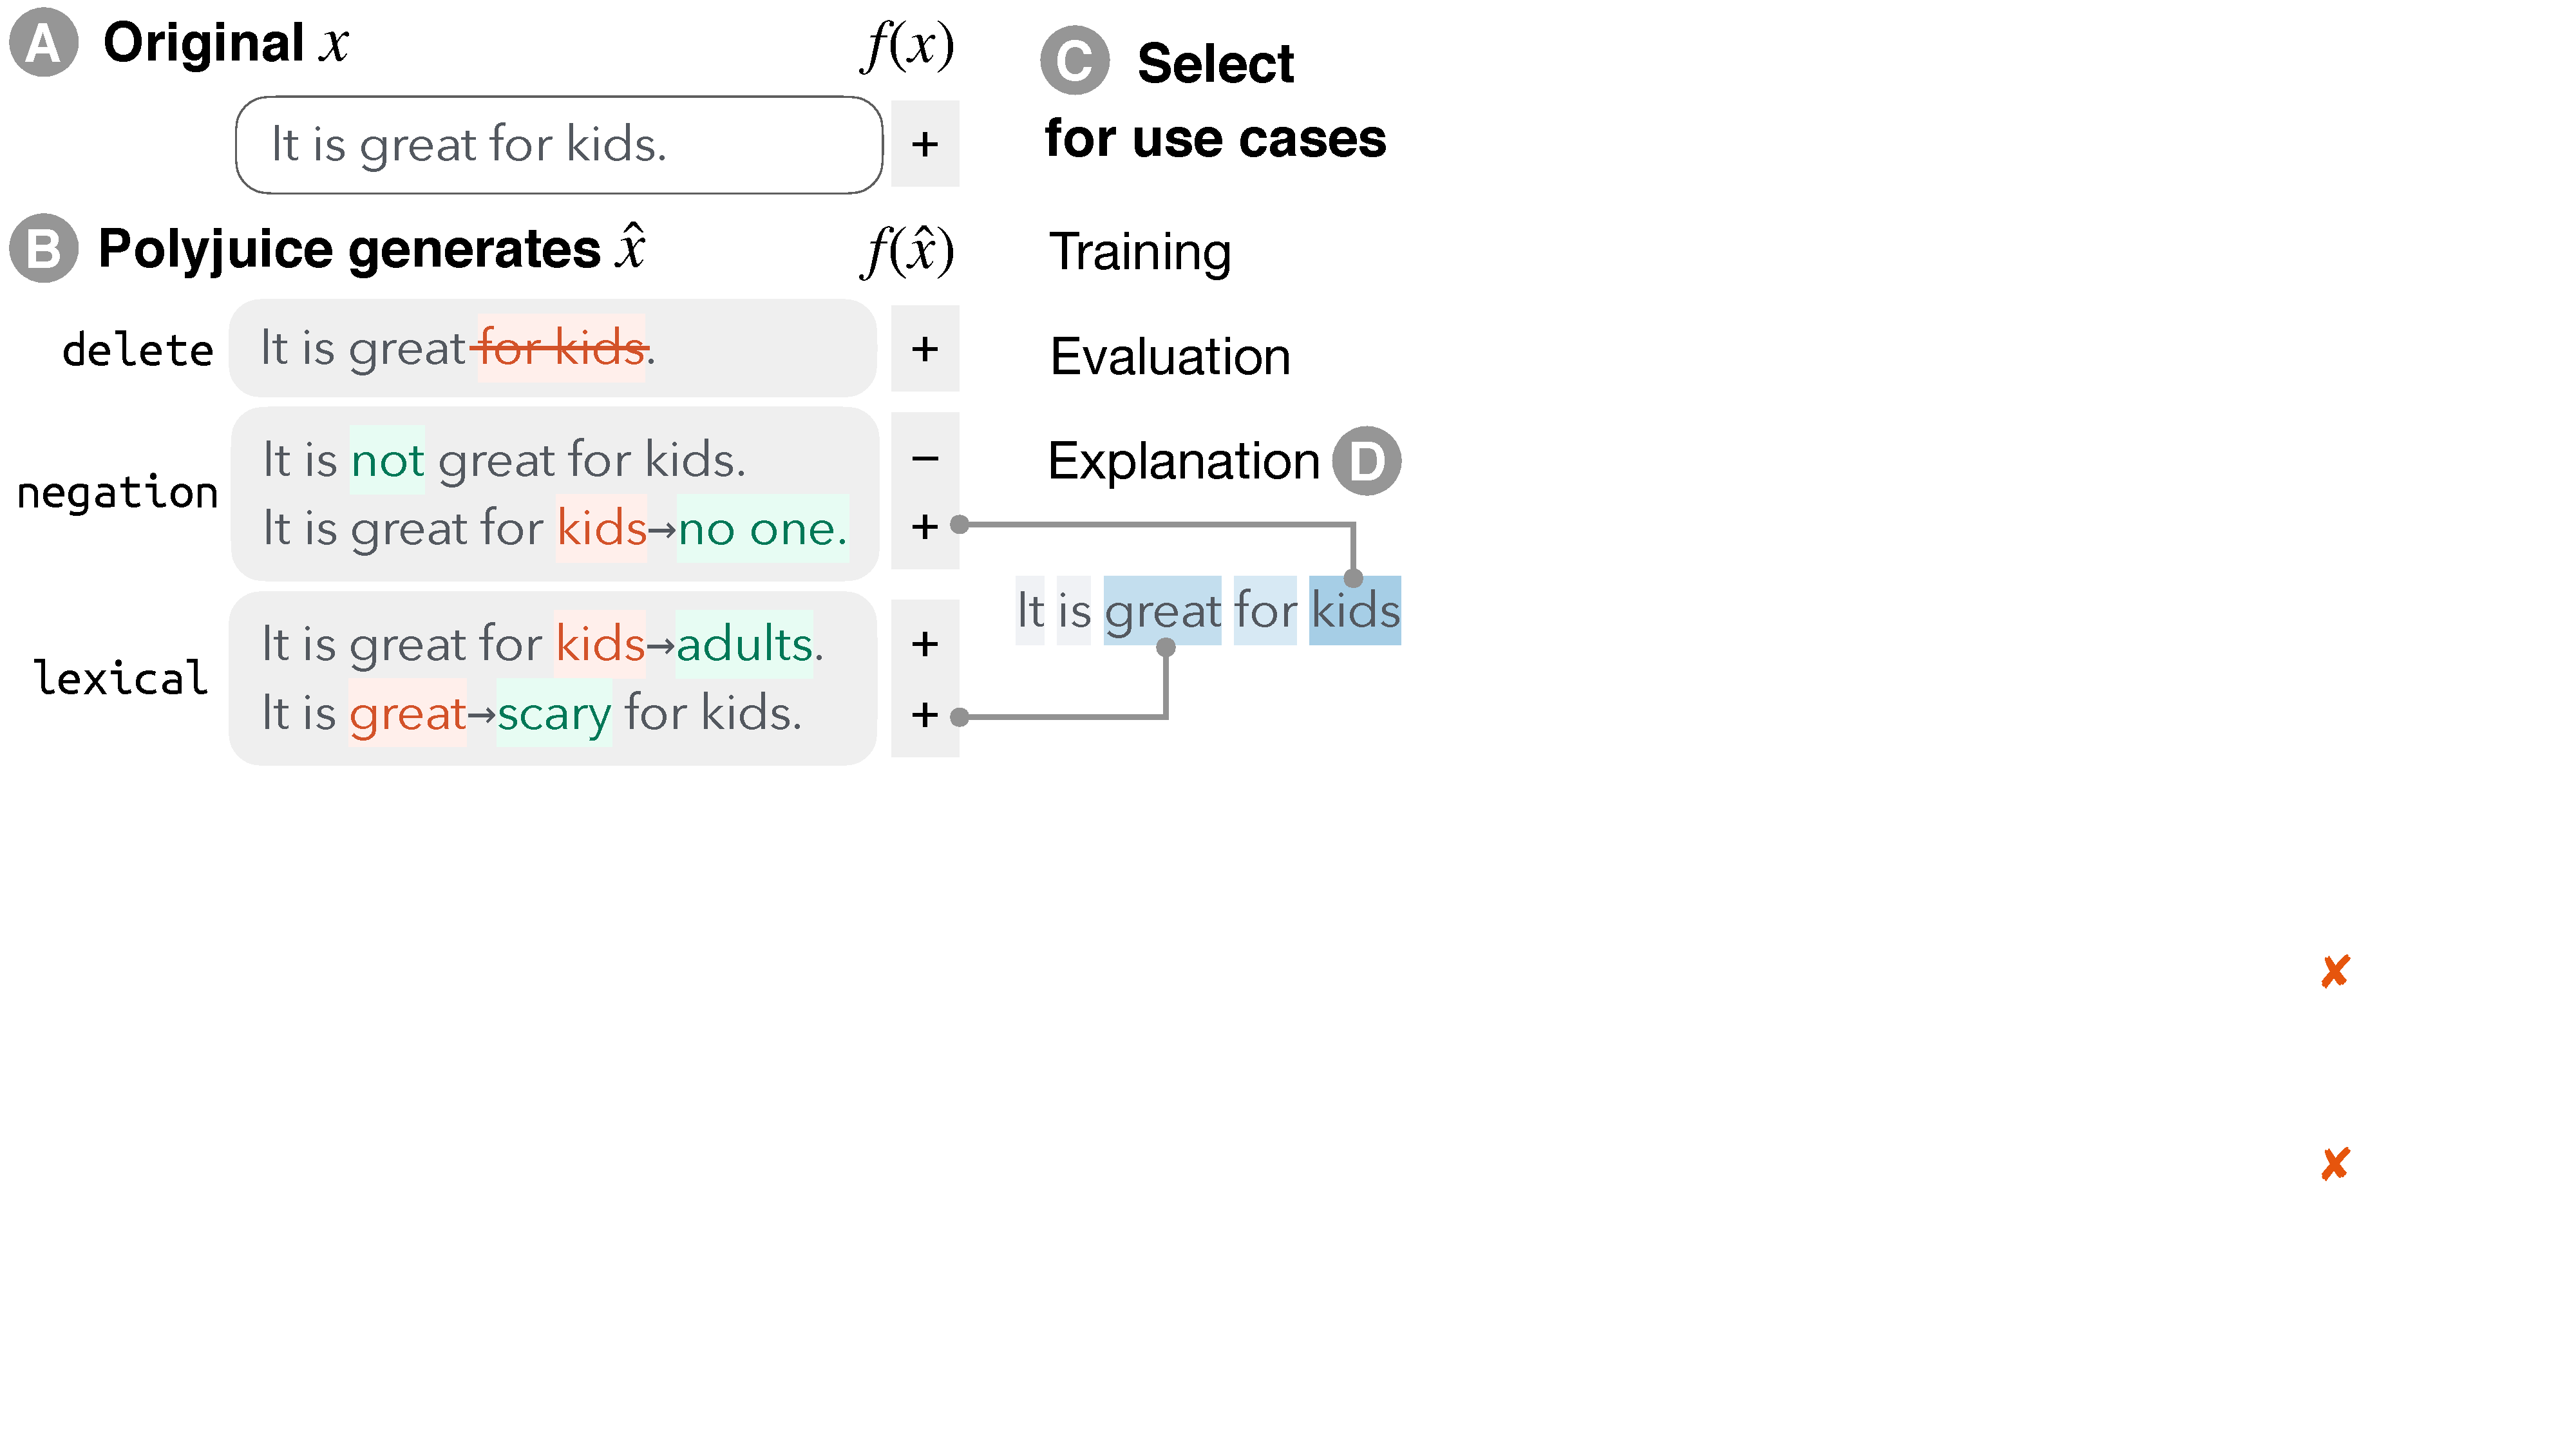
\includegraphics[width=1\columnwidth]{figures/teaser}
\vspace{-15pt}
\caption{Teaser of the idea. \wts{Placeholder; Probably shouldn't be just examples, given we already have a big table. Re-do to include the applications.}}
\vspace{-10pt}
\label{fig:teaser}
\end{figure}


We demonstrate the usefulness of \sysname in three applications. 
First, we verify that the perturbations is beneficial for training and evaluation data collection. 
In three NLP tasks --- sentiment analysis (\sst), duplicate question detection (\qqp), and natural language inference (\nli) --- we ask crowdworkers to label the generated multiple perturbations of the same original instance.
We observed that the labeling was more efficient than not only creating new perturbation examples, but also labeling new instances, as workers only need to parse the entire example once, and then process the labeling based on the changes.
\wts{Do we need to claim this, and do we need to verify this? Or maybe we can just say this is true in the labeling part, and do not claim *observing* it?}
Using the collected data as contrast sets~\cite{gardner2020contrast}, \ie evaluation dataset with minimal perturbations across the decision boundary, we observed that the performances of state-of-the-art models decrease significantly. 
Using the data for augmentation, we observed that the perturbation helps improve models' generalization accuracies on out-of-domain datasets, challenge sets and contrast sets, as well as CheckList testing results~\cite{checklist:acl20}, while maintaining the in-domain accuracy.

Second, we also use the perturbations to supply existing explanations methods.
We ``criticize'' existing feature attribution methods like SHAP~\cite{NIPS2017_7062} by selecting perturbations whose model prediction conflict with the corresponding token importance (\eg the model prediction changes when a supposedly insignificant feature is replaced.)
In a user study, we verify the surprise...

In summary, we contribute: 
\begin{compactenum}
\item A formalization of the perturbation task, with applications and desire properties extracted from existing literature.
\item A finetuned language model as perturbation generator, 
\item Demonstrations of perturbation usefulness on data augmentation, contrast set collection, and model explanation. 
\end{compactenum}





%Automated approahces using templates or word substitutions usually cover limited capabilities, whereas manual perturbations are usually expensive and hard to scale. 


%Another approach is to employ counterfactual reasoning: what would have happened if X was different? Many analysis and evaluation approaches rely on counterfactual reasoning, e.g. anchors, Errudite, SEARs, contrast sets, 'learning the difference that makes a difference', and counterfactual explanations in general. Some data augmentation approaches also rely on counterfactual reasoning, and focus on perturbing existing inputs rather than on getting new data. Intuitively, perturbations of inputs would allow us to highlight what really matters more efficiently than getting different examples (again, language is high dimensional).


\begin{comment}

prior work on counterfactual generation typically follows one of two extremes.
On the one hand, templates or perturbation rules (used by Errudite and Checklist) allow targeted inspections, but can only cover limited linguistic patterns.
On the other hand, those that thrive in diversity are either too uncontrolled (e.g., text generation~\cite{iyyer2018adversarial}) or hard to scale (e.g., manual rewrites~\cite{kaushik2019learning, gardner2020contrast}).



I seek to achieve a balance between control and generation diversity. 
To this end, I have fine-tuned language models for perturbation generation.

%Through intrinsic evaluation, we have found that our method works as we expect.
Moving forward, I plan to explore whether our method is helpful in various downstream tasks. 
First, the perturbations can potentially serve as extensive counterfactual explanations, i.e., explaining models' reaction to \emph{a set of changes}, rather than \emph{one change}~\cite{ribeiro2018semantically, ribeiro2018anchors, feder2020causalm}.
%We plan to use groups of perturbations as explanations, and suggests insightful groups to the practitioner based on certain predefined criteria.
A group of highly related changes may reveal model insufficiencies that are hard to spot otherwise (e.g., sentiment analysis model only recognizing certain kinds of negations like ``did not'', but misclassifying others like ``I would never.'')
%We plan to design a mixed-initiative method, where a system ranks groups of perturbations based on certain predefined criteria, and suggests the most insightful ones to the practitioner. 
%For example, minimal changes that affected the models' prediction possibly indicate the model is unstable.
%In turn, the practitioner can customize the exploration based on where or how s/he would like to inspect the model, and decide when to move to a different angle, or further drill down.
We plan to verify the insightfulness of these explanations through typical evaluation methods, e.g., surprise, simulatability~\cite{hase2020evaluating}.
Second, I hope to collect more effective contrast sets~\cite{gardner2020evaluating} that can reveal the vulnerability of the model.
I plan to annotate the generated perturbations with class labels in crowdsourcing tasks (e.g., positive or negative in sentiment analysis). 
%where a crowdworker label each sentence with a .%, or invalid (the sentence does not make sense, etc.). 
Then, to evaluate, I plan to verify whether we can find more bugs in the state-of-the-art models (i.e., if the accuracy further drops on these datasets).
Further, the data collected can be used for data augmentation~\cite{kaushik2019learning}. 
I plan to explore whether models trained with such perturbations can become more capable of handling certain capabilities (e.g., pass more tests in CheckList related to negation).
\end{comment}

